\epigraph{ 
    This remark is based on a ``theorem'', which as far as I know has never been proven, but which I cannot imagine could be wrong.
}
{
    Steven Weinberg, 1979~\autocite{weinbergPhenomenologicalLagrangians1979a}
}


Stars and planets have long been one of the main driving engines behind the developments of physics.
A lot of early mathematics was developed to predict the seasons, the phases of the moon and to navigate using the stars.
One of the most important confirmation of Newton's laws of motion and gravity was their prediction of Kepler's laws, the empirical observations of the orbits of planets around the Sun.
Likewise, the successor to Newton's law of gravitation, Einstein's general relativity, was first shown to be more accurate than its predecessor by predicting the drift of the perihelion of the orbit of Mercury~\autocite{carrollSpacetimeGeometryIntroduction2019}.
The radiation of the Sun has been part of the development of the theory of light and thermal radiation~\autocite{hemmerTermiskFysikk2002}.
To understand the process that fuels the Sun, we had to develop special relativity, in which mass is described as just another form of energy, as well as quantum mechanics and the theory of nuclear fusion.
Observations of the neutrinos which result from these processes were used to show the process of neutrino oscillations~\autocite{prialnikIntroductionTheoryStellar2000}.
Today, these are some of the only empirical data in physics that conflict with the standard model of particle physics.
The Sun might therefore still be part of the development of new fundamental physics.

Even after a star has depleted its fusion fuel it can remain an object of great interest.
Stars with less mass than around $10$ times that of the earth, $M_\odot$, will towards the end of their active life shed most of their outer layers, leaving behind an inert white-hot mass only supported by the degeneracy pressure of electrons.
These are called \emph{white dwarves}.
One cubic centimeter of the material that makes up white dwarves weighs more than a ton.
Sirius B, the fainter companion to Sirius is a white dwarf.
Type Ia supernovae happen as white dwarves reach their upper mass limit, the Chandrasekhar limit, and are invaluable in mapping the distance of our universe~\autocite{carrollSpacetimeGeometryIntroduction2019}.
White dwarves, together with the even more dense \emph{neutron stars} collectively known as \emph{compact stars}.
Neutron stars are left after the supernova explosions of massive stars~\autocite{prialnikIntroductionTheoryStellar2000}.
They were first predicted solely on theoretical backgrounds, and later discovered in the form of pulsars, rotating neutron stars with frequencies below a tenth of a second which strong magnetic fields acting as particle accelerators~\autocite{prialnikIntroductionTheoryStellar2000},
Compact stars are some of the most environments in our universe, and as such, they are excellent places for exotic physics to happen.

Recently, a new form of compact stars has been proposed, called pion stars~\autocite{andersenBoseEinsteinCondensationPion2018,brandtNewClassCompact2018,carignanoScrutinizingPionCondensed2017}.
These stars are composed of a pion condensate.
The pion particles are bosons, in contrast to electrons and neutrons, which are fermions.
The pressure in pion stars must therefore be maintained by repulsive interactions, unlike in neutron stars and white dwarves, where it is due to the Pauli exclusion principle.
In this thesis, we will develop chiral perturbation theory, a model for the dynamics of pions and the other pseudoscalar mesons, in order to investigate the properties of pion stars.
This involves a survey of the theoretical foundations and thermodynamic calculations.
Pion stars are yet only a theoretical proposal, although if history is to be of any guidance, that does not mean there aren't valuable insights to be gained from researching them.




\section{The standard model, QCD, and effective theories}


The standard model of particle physics is the totality of everything particle physicists are confident they understand concerning the fundamental building blocks of our universe.
It is arguably the most successful scientific theory of all time and makes fantastically accurate predictions of the behavior of fundamental particles and
in combination with general relativity, and Einstein's theory of gravity, it is, for now, our best answer to how the world works.
The standard model is a quantum field theory (QFT) and describes both the elementary matter particles and the forces between them as excitations in underlying fields, which permeate all space-time.
If we include the masses of neutrinos in the standard model, it has 26 free parameters~\autocite{kramerStandardModelParticle2017}.
The particles of the standard model are illustrated in \autoref{fig: standard model}~\autocite{griffithsIntroductionElementaryParticles2008,schwartzQuantumFieldTheory2013}


\begin{figure}[!htb]
    \centering
    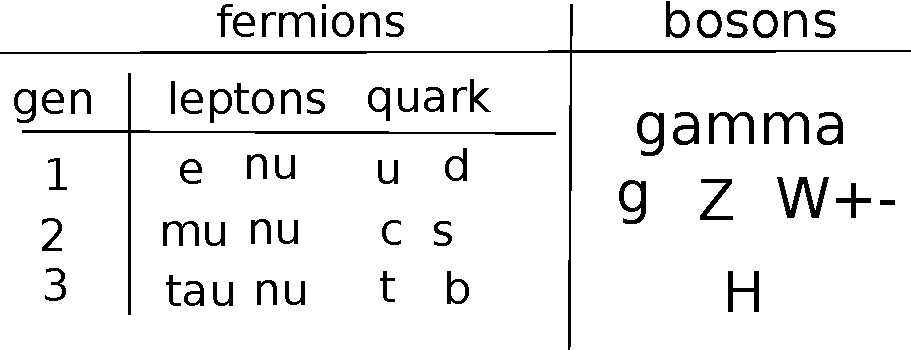
\includegraphics[width=.75\textwidth]{figurer/standard_model.pdf}
    \caption{The particles of the standard model}
    \label{fig: standard model}
\end{figure}




\section{Units}
\label{section: units}


In this thesis, we employ \emph{natural units}, defined by
%
\begin{equation}
    \hbar = c = k_B = 1,
\end{equation}
%
where $\hbar$ is Planck's reduced constant, $c$ is the speed of light, and $k_B$ is Boltzmann's constant.
Dimensionfull results are often given in $\text{MeV}$.
Uncertainties are indicated when the precision is less than four significant figures. 
However, the central value is always used in calculations.
All values in this section are from the Particle Data Group~\cite{particledatagroupReviewParticlePhysics2020}.
To obtain results in the SI-system, we use the following conversion factors, as given by
%
\begin{align}
    \label{speed of ligh}
    c       &= 2.998 \cdot 10^8     \, \text{m} \, \text{s}^{-1}, \\
    \label{hbar}
    \hbar   &= 1.055 \cdot 10^{-34} \, \text{J} \, \text{s}, \\
    \label{Boltzmanns constat}
    k_B     &= 1.380 \cdot 10^{-23} \, \text{J} \, \text K^{-1}, \\
    \label{Newtons gravitational constant}
    G       &= 6.674 \cdot 10^{-11} \, \text m^3 \, \text{kg}^{-1} \, \text s^{-2},
\end{align}
%
where $G$ is Newton's gravitational constant.
The conversion factor between $\text{MeV}$ and SI-units is
%
\begin{equation}
    \label{electronvolt}
    1 \, \text{MeV} = 1.60218\, \cdot 10^{-19} \, \text{J}. 
\end{equation}
%
The fine structure constant and the elementary charge is
%
\begin{align}
    \label{Fine structure constant}
    \alpha &= 7.297 \cdot 10^{-3}, \\
    \label{Elementary charge}
    e &:= \sqrt{4 \pi \alpha} =  3.028\cdot 10^{-1}.
\end{align}
%
In astronomical calculation, the solar mass is used, which is
%
\begin{equation}
    \label{solar mass}
    M_\odot = 1.988 \cdot 10^{30} \, \text{kg}.
\end{equation}
%
The physical parameters we use are
%
\begingroup
\allowdisplaybreaks % Make page break possbible
\begin{align}
    \label{pion decay constant}
    f_\pi & =  92.1 \, \text{MeV}, \\
    \label{pion mass}
    m_\pio & = 134.98 \, \text{MeV}, \\
    \label{charged pion mass}
    m_{\pipm} &= 139.57 \, \text{MeV}, \\
    m_{\Kpm} & = 493.68\,\text{MeV}, \\
    m_{\Ko} & = 497.61\,\text{MeV}, \\
    m_e &= 0.5110 \, \text{MeV}, \\
    m_\mu &= 105.7 \, \text{MeV}, \\
    \label{mass of neutron}
    m_N &= 939.57 \, \text{MeV}.
\end{align}
\endgroup

To make this thesis as self-contained as possible, we have included some parts from the earlier specialization project, with minor modifications.
These sections are marked with an asterisk in the table of content.
